\scanpage{16}
\diagram{\begin{tikzcd}[ampersand replacement=\&,column sep=large]
\operatorname{Ens}(\pi)\arrow[r,"F_X","{}_{\pi'}X_\pi"']\&\operatorname{Ens}(\pi')\arrow[r,"F_Y","{}_{\pi''}Y_{\pi'}"']\&\operatorname{Ens}(\pi'')
%
\end{tikzcd}}
\[
F_Y\circ F_X=F_{Y\wedge_{\pi'}X}
\]
\figure{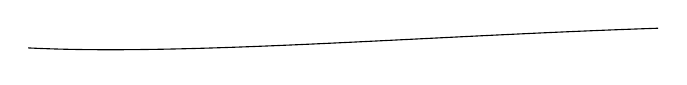
\begin{tikzpicture}\draw (0,0)..controls(2,-.1)and(5,.15)..(8,.25);\end{tikzpicture}}

${}_{\pi'}X_\pi$ bitorseur; \unsure{classifier} à isom près ?

\[
\pi'\xrightarrow{\sim}{}^X\pi
\overset{\substack{\text{non can.}\\\text{mais can. dans }\operatorname{Isomext}({}^X\pi,\pi)}}{\simeq}\pi
\]

Donc $X$ définit $\operatorname{Isomext}(\pi',\pi)$

\deleted{\unsure{Cl d'i.} de bit $(\pi',\pi)$}
\[
\pi_0\bigl(\underline{\operatorname{Bit}}(\pi',\pi)\bigr)
\xrightarrow{\sim}\operatorname{Isomext}(\pi',\pi)
\]

\diagram{\begin{tikzcd}[ampersand replacement=\&,column sep=large,row sep=huge]
\pi_0\bigl(\underline{\unsure{\operatorname{Bitpt}}}(\pi',\pi)\bigr)\arrow[r,phantom,"\simeq"]\arrow[d]\&\operatorname{Isom}(\pi',\pi)\arrow[dl,"\begin{gathered}\unsure{\text{surj.}}\\\unsure{\text{passage au quotient}}\\\text{par }\operatorname{Int}(\pi)\end{gathered}"]\\
\pi_0\bigl(\underline{\operatorname{Bit}}(\pi',\pi)\bigr)\simeq\operatorname{Isom}(\pi',\pi)/\operatorname{Int}(\pi)=\operatorname{Isomext}(\pi',\pi)\&
\end{tikzcd}}

\figure{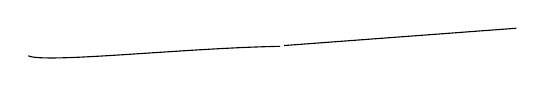
\begin{tikzpicture}\draw (0,0)..controls(.2,-.1)and(2,.1)..(3.2,.12);\draw (3.25,.13)--(6.2,.35);\end{tikzpicture}}

\diagram{\begin{tikzcd}[ampersand replacement=\&,column sep=large]
F^2\arrow[r,"\sim","\mu"']\&\operatorname{id}
\end{tikzcd}}
\diagram{\begin{tikzcd}[ampersand replacement=\&,column sep=large]
F(F(E))\arrow[r,"\mu_E"]\&E
\end{tikzcd}}
\diagram{\begin{tikzcd}[ampersand replacement=\&,column sep=large]
F(F(\underline{F(E)}))\arrow[r,shift left=2,"F(\mu_E)"]\arrow[r,shift right=2,"\mu_{F(E)}"']\&F(E)
\end{tikzcd}}
\[
\unsure{F\mu|F\circ\mu}=\mu\mathbin{\unsure{\cdot|\star}}F:F^3\longrightarrow F
\]

\mspage{15}
